% =============================================================================
% CHAPTER 4 — THE PROPOSED METHOD: PATHCAST
% Thesis: PATHCAST
% Version: REDUCED — paraphrase paragraphs and meta-summaries removed.
%          All formal content (definitions, algorithms, theorems, properties)
%          preserved. Cross-references unchanged.
% =============================================================================

\chapter{The Proposed Method: PATHCAST}
\label{ch:method}

This chapter presents the formal specification of the proposed method,
PATHCAST. The method integrates process mining, Markov chain estimation,
Monte Carlo simulation, and machine learning into a unified pipeline that
transforms heterogeneous software repository data into probabilistic
process forecasts.

Section~\ref{sec:method-overview} provides the architectural overview and
defines the formal pipeline. Sections~\ref{sec:stage1}
through~\ref{sec:stage4} formalize each pipeline stage with input/output
contracts, algorithms, and correctness properties.
Section~\ref{sec:ml-component} specifies the machine learning enhancement
component. Section~\ref{sec:integration} formalizes the inter-stage data
contracts. Section~\ref{sec:method-properties} establishes the formal
properties and theoretical guarantees.
Section~\ref{sec:method-summary} synthesizes the contributions.


% =============================================================================
% 4.1 METHOD OVERVIEW
% =============================================================================
\section{Architectural Overview}
\label{sec:method-overview}

\subsection{Pipeline Definition}
\label{sec:pipeline-def}

PATHCAST is defined as a composition of four sequential transformation
stages and one parallel enhancement component:

\begin{definition}[PATHCAST Pipeline]
\label{def:pipeline}
The PATHCAST pipeline is a function composition:
\begin{equation}
\label{eq:pipeline}
\mathcal{F} = \mathcal{S}_4 \circ \mathcal{S}_3 \circ \mathcal{S}_2 \circ \mathcal{S}_1
\end{equation}
where:
\begin{align}
\mathcal{S}_1 &: \mathcal{R} \to \mathcal{L}
    && \text{(Event Log Construction)} \label{eq:stage1-sig} \\
\mathcal{S}_2 &: \mathcal{L} \to (M, \Phi)
    && \text{(Process Mining)} \label{eq:stage2-sig} \\
\mathcal{S}_3 &: (\mathcal{L}, M) \to (P, N, B, \hat{F})
    && \text{(Markov Estimation)} \label{eq:stage3-sig} \\
\mathcal{S}_4 &: (P, \hat{F}, s_0, M_{\text{sim}}) \to \hat{\mathcal{D}}
    && \text{(Monte Carlo Simulation)} \label{eq:stage4-sig}
\end{align}
and a parallel component:
\begin{equation}
\mathcal{S}_{\text{ML}} : (\mathcal{L}, \Phi, P, N) \to \hat{f}
    \quad \text{(ML Enhancement)} \label{eq:ml-sig}
\end{equation}
\end{definition}

The notation: $\mathcal{R}$ denotes software repositories; $\mathcal{L}$
the structured event log; $M$ the discovered process model; $\Phi$ the
process metrics vector; $P$ the Markov transition matrix; $N$ the
fundamental matrix; $B$ the absorption probability matrix; $\hat{F}$ the
empirical sojourn time distributions; $\hat{\mathcal{D}}$ the empirical
forecast distribution; $\hat{f}$ the trained ML predictor.

\subsection{Pipeline Architecture}
\label{sec:pipeline-arch}

Figure~\ref{fig:pipeline-architecture} illustrates the complete pipeline
architecture with data flows between stages.

\begin{figure}[htbp]
\centering
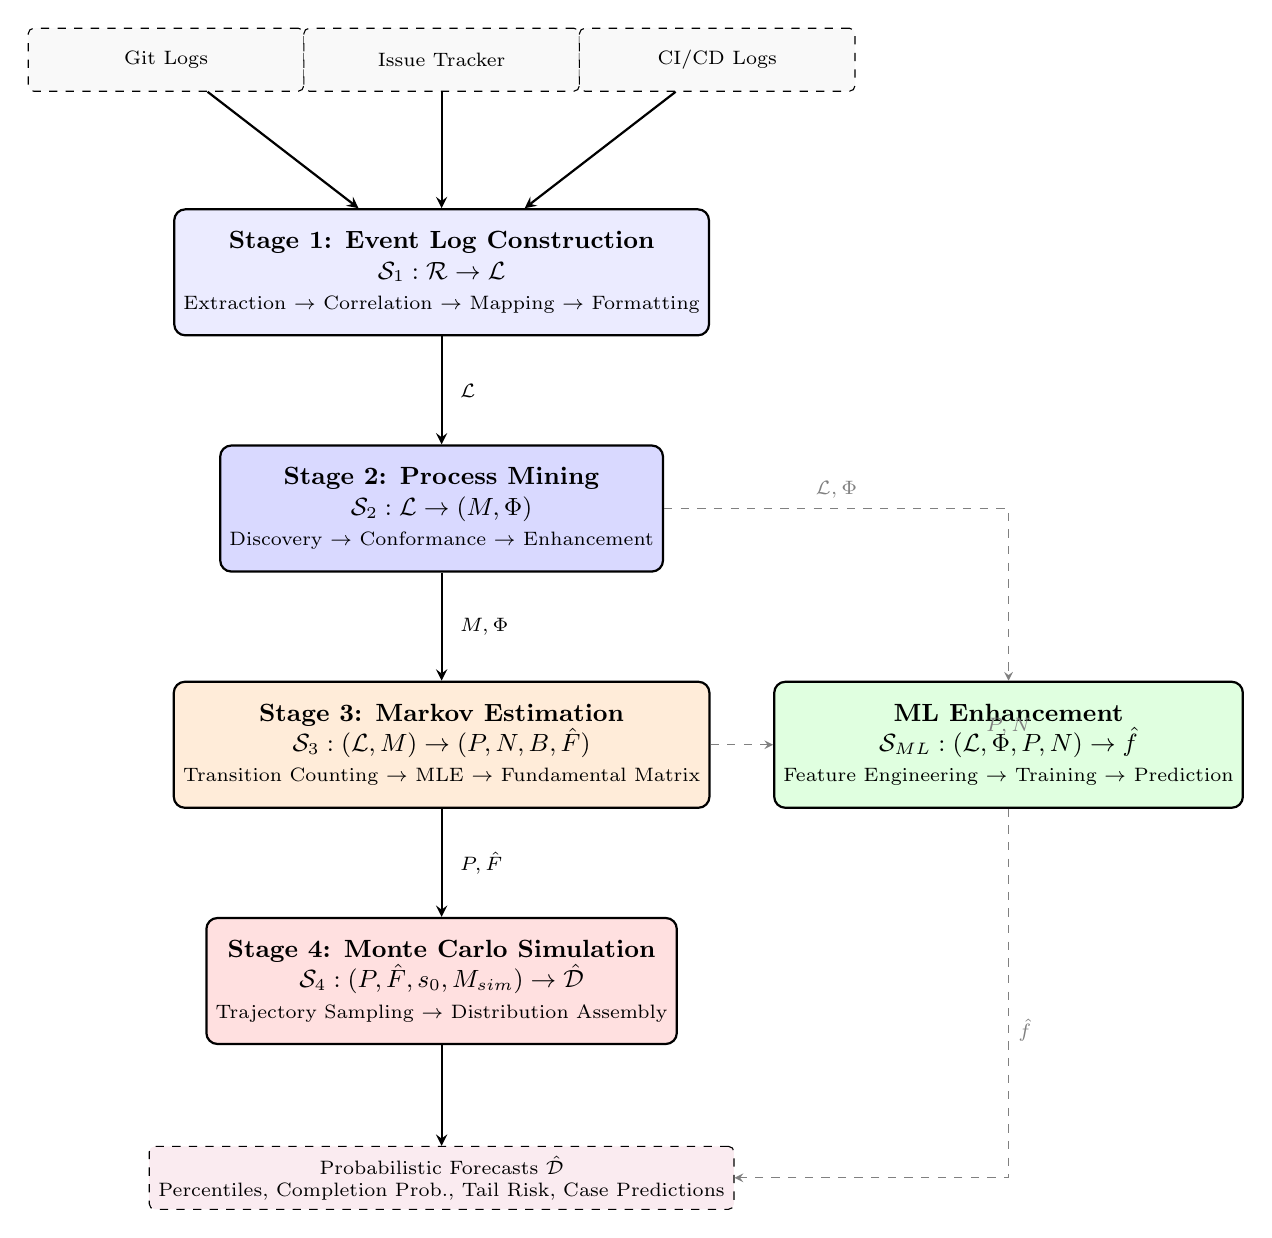
\begin{tikzpicture}[
    node distance=2.2cm,
    stage/.style={rectangle, draw, thick, rounded corners=4pt,
                  minimum width=5.5cm, minimum height=1.6cm,
                  align=center, font=\small},
    data/.style={rectangle, draw, dashed, rounded corners=2pt,
                 minimum width=3.5cm, minimum height=0.8cm,
                 align=center, font=\scriptsize, fill=gray!5},
    arrow/.style={->, thick, >=stealth},
    darrow/.style={->, dashed, >=stealth, gray},
    lbl/.style={font=\scriptsize, midway, right, xshift=3pt}
]
    \node[data] (git) at (-3.5, 0) {Git Logs};
    \node[data] (jira) at (0, 0) {Issue Tracker};
    \node[data] (ci) at (3.5, 0) {CI/CD Logs};

    \node[stage, fill=blue!8, below of=jira, yshift=-0.5cm] (s1) {
        \textbf{Stage 1: Event Log Construction}\\
        $\mathcal{S}_1 : \mathcal{R} \to \mathcal{L}$\\
        {\scriptsize Extraction $\to$ Correlation $\to$ Mapping $\to$ Formatting}
    };

    \node[stage, fill=blue!15, below of=s1, yshift=-0.8cm] (s2) {
        \textbf{Stage 2: Process Mining}\\
        $\mathcal{S}_2 : \mathcal{L} \to (M, \Phi)$\\
        {\scriptsize Discovery $\to$ Conformance $\to$ Enhancement}
    };

    \node[stage, fill=orange!15, below of=s2, yshift=-0.8cm] (s3) {
        \textbf{Stage 3: Markov Estimation}\\
        $\mathcal{S}_3 : (\mathcal{L}, M) \to (P, N, B, \hat{F})$\\
        {\scriptsize Transition Counting $\to$ MLE $\to$ Fundamental Matrix}
    };

    \node[stage, fill=red!12, below of=s3, yshift=-0.8cm] (s4) {
        \textbf{Stage 4: Monte Carlo Simulation}\\
        $\mathcal{S}_4 : (P, \hat{F}, s_0, M_{\text{sim}}) \to \hat{\mathcal{D}}$\\
        {\scriptsize Trajectory Sampling $\to$ Distribution Assembly}
    };

    \node[stage, fill=green!12, right of=s3, xshift=5cm] (ml) {
        \textbf{ML Enhancement}\\
        $\mathcal{S}_{\text{ML}} : (\mathcal{L}, \Phi, P, N) \to \hat{f}$\\
        {\scriptsize Feature Engineering $\to$ Training $\to$ Prediction}
    };

    \node[data, below of=s4, yshift=-0.3cm, minimum width=5.5cm, fill=purple!8] (output) {
        Probabilistic Forecasts $\hat{\mathcal{D}}$\\
        {\scriptsize Percentiles, Completion Prob., Tail Risk, Case Predictions}
    };

    \draw[arrow] (git) -- (s1);
    \draw[arrow] (jira) -- (s1);
    \draw[arrow] (ci) -- (s1);
    \draw[arrow] (s1) -- (s2) node[lbl] {$\mathcal{L}$};
    \draw[arrow] (s2) -- (s3) node[lbl] {$M, \Phi$};
    \draw[arrow] (s3) -- (s4) node[lbl] {$P, \hat{F}$};
    \draw[arrow] (s4) -- (output);

    \draw[darrow] (s2) -| (ml) node[font=\scriptsize, above, pos=0.25] {$\mathcal{L}, \Phi$};
    \draw[darrow] (s3) -- (ml) node[font=\scriptsize, above] {$P, N$};
    \draw[darrow] (ml) |- (output) node[font=\scriptsize, right, pos=0.3] {$\hat{f}$};

\end{tikzpicture}
\caption{PATHCAST pipeline architecture. Solid arrows indicate the
primary sequential pipeline; dashed arrows indicate ML enhancement data flows.}
\label{fig:pipeline-architecture}
\end{figure}


\subsection{Design Principles}
\label{sec:design-principles}

The pipeline architecture is governed by three design principles:

\textbf{Principle 1 (Empirical Grounding).} Every model parameter is
estimated from observed data, never assumed \emph{a priori}. The transition
matrix $P$ is estimated from event log counts; sojourn distributions
$\hat{F}$ are constructed from observed timestamps; ML features are
extracted from empirical traces. No distributional assumptions are imposed
unless empirically validated.

\textbf{Principle 2 (Stage Composability).} Each stage has a formally
defined input/output contract (Definitions~\ref{def:contract-s1}
through~\ref{def:contract-s4}). Stages can be independently tested,
replaced, or extended without affecting other stages, provided the
contract is preserved.

\textbf{Principle 3 (Distributional Outputs).} The pipeline produces
probability distributions, not point estimates. Every forecast is a
collection of $M_{\text{sim}}$ simulated outcomes from which percentiles,
intervals, and tail probabilities are extracted.


\subsection{Component View}
\label{sec:spaf-overview}

\begin{figure}
    \centering
    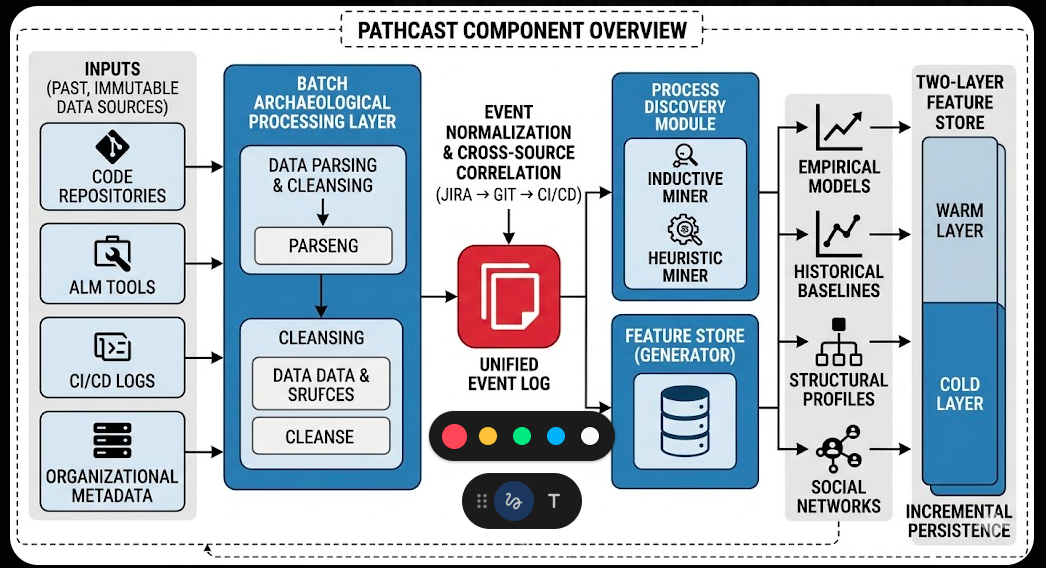
\includegraphics[width=1\linewidth]{figures/path-cast-component-overview.png}
    \caption{PATHCAST component overview.}
    \label{fig:pathcast-architecture}
\end{figure}

Figure~\ref{fig:pathcast-architecture} presents the component view of
PATHCAST; this view focuses on the historical-data processing layer that
precedes forecasting (the past-facing portion of the pipeline that builds
the models later used to project the future). The framework
ingests historical, immutable data sources (code repositories, ALM tools,
CI/CD logs, organizational metadata) through a batch archaeological
processing layer. The pipeline produces a unified event log through event
normalization and cross-source correlation
(Jira~$\to$~Git~$\to$~CI/CD), feeding both the process discovery module
(Inductive Miner, Heuristic Miner) and the feature store. Outputs of the
PATHCAST component---empirical models, historical baselines, structural
profiles, and (optionally) organizational social-network features---are
persisted incrementally in a two-layer feature store (cold and warm) that
serves as input for the forecasting stages described in
Sections~\ref{sec:stage2} through~\ref{sec:stage4}. The social-network
features are an optional input to the machine-learning enhancement
component (Section~\ref{sec:ml-component}) and are not required by the core
process-aware forecasting pipeline; they are included here for architectural
completeness and may be omitted without affecting Stages~1--4.

Figure~\ref{fig:pathcast-architecture} is the \emph{architectural
realization} of the method: it shows implementation concerns such as the
cold/warm feature store and the persistence layer. The \emph{functional
abstraction} of the method---the mathematical mapping from repositories to
forecast distributions---is given by the stage contracts of
Section~\ref{sec:stage-contracts}, in which the feature store is the
persistence mechanism for the formally specified stage outputs
$(\mathcal{L}, M, \Phi, S, P, N, B, \hat{F})$ rather than an additional
formal object. The fundamental matrix $N$ and absorption matrix $B$
produced by Stage~3, in particular, are consumed by the machine-learning
component as predictive features (see the $\mathrm{S3}\to\mathrm{ML}$
contract in Table~\ref{tab:data-contracts}), not merely computed for
descriptive analysis.


\subsection{Stage Contracts}
\label{sec:stage-contracts}

Each stage of the pipeline is specified by an input/output contract with
pre- and postconditions; the contracts are gathered here once and
referenced---rather than restated---in the stage sections that follow.
Stage composability (Principle~2) depends on these contracts: stages may
be independently replaced or extended as long as their contracts are
preserved.

\begin{definition}[Stage 1 Contract]
\label{def:contract-s1}
\textbf{Input:} repositories $\mathcal{R} = \{r_1, \ldots, r_n\}$, each
$r_i$ a set of time-ordered raw-event streams $\{D_i^{(j)}\}$.
\textbf{Output:} structured event log
$\mathcal{L} = \{\sigma_c \mid c \in \mathcal{C}\}$ satisfying
Definition~\ref{def:event-log}.
\textbf{Postconditions:} every event has a valid case identifier,
activity name and timestamp; events are timestamp-ordered within each
trace; activity names belong to the SDLC taxonomy $\mathcal{A}$.
$\mathcal{S}_1 = \textsc{Format} \circ \textsc{Map} \circ
\textsc{Correlate} \circ \textsc{Extract}$
(Equation~\ref{eq:s1-decomposition}).
\end{definition}

\begin{definition}[Stage 2 Contract]
\label{def:contract-s2}
\textbf{Input:} an event log $\mathcal{L}$ satisfying
Definition~\ref{def:contract-s1}.
\textbf{Output:} a triple $(M, \Phi, S)$ with discovered model $M$,
metrics vector
$\Phi = (\phi_{\text{fit}}, \phi_{\text{prec}}, \phi_{\text{gen}},
\phi_{\text{perf}})$, and state space $S = (S_T, S_A)$.
\textbf{Postconditions:} $M$ is sound;
$\phi_{\text{fit}}, \phi_{\text{prec}} \in [0,1]$; $\phi_{\text{perf}}$
contains per-activity sojourn statistics; $|S_T|\geq 1$ and $|S_A|\geq 1$;
every $a \in \mathcal{A}$ observed in $\mathcal{L}$ maps to exactly one
state.
\end{definition}

\begin{definition}[Stage 3 Contract]
\label{def:contract-s3}
\textbf{Input:} $\mathcal{L}$ and $S = S_T \cup S_A$.
\textbf{Output:} $(P, N, B, \hat{F}, \pi)$ with transition matrix
$P \in \mathbb{R}^{|S|\times|S|}$, fundamental matrix
$N = (I-Q)^{-1} \in \mathbb{R}^{|S_T|\times|S_T|}$, absorption matrix
$B = NR \in \mathbb{R}^{|S_T|\times|S_A|}$, sojourn distributions
$\hat{F} = \{\hat{F}_s\}_{s \in S_T}$, and stationary distribution $\pi$.
\textbf{Preconditions:} $|S_T| \geq 1$, $|S_A| \geq 1$, every transient
state has at least one observed outgoing transition.
\textbf{Postconditions:} $P$ row-stochastic; $(I-Q)$ invertible;
$N_{ij} \geq 0$; $\sum_j B_{ij} = 1$; each $\hat{F}_s$ has at least
$n_{\min}$ observations.
$\mathcal{S}_3 = \textsc{Stationary} \circ \textsc{Sojourn} \circ
\textsc{Absorb} \circ \textsc{Estimate} \circ \textsc{Count}$
(Equation~\ref{eq:s3-decomposition}).
\end{definition}

\begin{definition}[Stage 4 Contract]
\label{def:contract-s4}
\textbf{Input:} $P$, $\hat{F}$, initial state $s_0$ (or initial
distribution $\pi_0$), and the simulation budget
$M_{\text{sim}} \in \mathbb{N}$.
\textbf{Output:} the empirical forecast distribution
$\hat{\mathcal{D}} = \{(T^{(m)}, o^{(m)}, \psi^{(m)})\}_{m=1}^{M_{\text{sim}}}$
of lead times, terminal states and trajectories
(Equation~\ref{eq:forecast-distribution}).
\textbf{Postconditions:} $|\hat{\mathcal{D}}| = M_{\text{sim}}$, every
trajectory absorbs, $T^{(m)} > 0$.
\end{definition}

\begin{definition}[ML Component Contract]
\label{def:contract-ml}
\textbf{Input:} $\mathcal{L}$, $\Phi$, $P$, $N$.
\textbf{Output:} trained predictor $\hat{f}$ and feature importance
vector $\mathbf{w}$.
\textbf{Postconditions:} $\hat{f}$ is evaluated on a temporally disjoint
test set; AUC-ROC, F1, Brier score, MAE and MAPE are reported; $\mathbf{w}$
ranks features.
\end{definition}


% =============================================================================
% 4.2 STAGE 1: EVENT LOG CONSTRUCTION
% =============================================================================
\section{Stage 1: Event Log Construction}
\label{sec:stage1}

Stage 1 transforms heterogeneous software repository data into structured
event logs suitable for process mining.

Stage 1 satisfies the contract of
Definition~\ref{def:contract-s1}; the decomposition is
\begin{equation}
\label{eq:s1-decomposition}
\mathcal{S}_1 = \textsc{Format} \circ \textsc{Map} \circ \textsc{Correlate} \circ \textsc{Extract},
\end{equation}
detailed in the four subsections that follow.


\subsection{Event Extraction}
\label{sec:s1-extraction}

\begin{definition}[Raw Event]
\label{def:raw-event}
A raw event is a tuple $e^{\text{raw}} = (ts, src, type, payload)$ with
timestamp, source, type, and source-specific attribute map.
\end{definition}

\begin{definition}[Source Extractors]
\label{def:extractors}
\begin{align}
\textsc{Extract}_{\text{git}}    &: D^{(\text{git})} \to \{e^{\text{raw}}\}  \\
\textsc{Extract}_{\text{jira}}   &: D^{(\text{jira})} \to \{e^{\text{raw}}\} \\
\textsc{Extract}_{\text{ci}}     &: D^{(\text{ci})} \to \{e^{\text{raw}}\}   \\
\textsc{Extract}_{\text{review}} &: D^{(\text{review})} \to \{e^{\text{raw}}\}
\end{align}
\end{definition}

The raw event pool is
$E^{\text{raw}} = \bigcup_{i,j} \textsc{Extract}_{src(D_i^{(j)})}(D_i^{(j)})$.

Table~\ref{tab:event-extraction} specifies the extraction mapping per
source type.

\begin{table}[htbp]
\centering
\caption{Event extraction mapping per data source.}
\label{tab:event-extraction}
\small
\begin{tabular}{llll}
\toprule
\textbf{Source} & \textbf{Raw Event Type} & \textbf{Timestamp Source} & \textbf{Key Payload} \\
\midrule
Git    & \texttt{commit}            & Author date         & hash, author, files \\
       & \texttt{merge}             & Committer date      & branches \\
\midrule
Jira   & \texttt{status\_change}    & Changelog timestamp & from/to status \\
       & \texttt{created}           & Creation timestamp  & reporter, type \\
       & \texttt{assigned}          & Changelog timestamp & assignee \\
\midrule
CI/CD  & \texttt{build\_start}      & Build start         & pipeline, branch \\
       & \texttt{build\_end}        & Build end           & result, duration \\
       & \texttt{deploy}            & Deploy timestamp    & environment \\
\midrule
Review & \texttt{pr\_opened}        & PR creation         & author, base \\
       & \texttt{review\_submitted} & Review timestamp    & reviewer, decision \\
       & \texttt{pr\_merged}        & Merge timestamp     & merge method \\
       & \texttt{pr\_closed}        & Close timestamp     & reason \\
\bottomrule
\end{tabular}
\end{table}


\subsection{Case Correlation}
\label{sec:s1-correlation}

\begin{definition}[Case Correlation Function]
\label{def:correlation}
$\kappa : E^{\text{raw}} \to \mathcal{C} \cup \{\bot\}$, where $\bot$
indicates uncorrelated events.
\end{definition}

The correlation function is implemented as a cascade of strategies, applied
in order of decreasing specificity (Algorithm~\ref{alg:correlation}).

\begin{algorithm}[htbp]
\caption{Case Correlation Cascade}
\label{alg:correlation}
\begin{algorithmic}[1]
\REQUIRE Raw event pool $E^{\text{raw}}$, correlation configuration $\mathcal{K}$
\ENSURE Case-annotated event set $E^{\text{corr}} \subseteq E^{\text{raw}} \times \mathcal{C}$
\STATE Initialize $E^{\text{corr}} \gets \emptyset$, $E^{\text{pending}} \gets E^{\text{raw}}$
\FOR{each strategy $\kappa_k \in \mathcal{K}$ in priority order}
    \FOR{each event $e \in E^{\text{pending}}$}
        \STATE $c \gets \kappa_k(e)$
        \IF{$c \neq \bot$}
            \STATE $E^{\text{corr}} \gets E^{\text{corr}} \cup \{(e, c)\}$
            \STATE $E^{\text{pending}} \gets E^{\text{pending}} \setminus \{e\}$
        \ENDIF
    \ENDFOR
\ENDFOR
\STATE Report $|E^{\text{pending}}|$ uncorrelated events
\RETURN $E^{\text{corr}}$
\end{algorithmic}
\end{algorithm}

\textbf{Strategy $\kappa_1$ (Explicit Reference):} extracts issue keys from
structured fields (Jira issue key, Git commit message regex, GitHub PR
links). Formally:
\begin{equation}
\label{eq:kappa1}
\kappa_1(e) = \begin{cases}
    \text{issue\_key}(e.\text{payload}) & \text{if extractable} \\
    \bot & \text{otherwise}
\end{cases}
\end{equation}

\textbf{Strategy $\kappa_2$ (Structural Link):} platform-provided
relationships (PR$\to$issue, build$\to$commit, sub-task$\to$parent).

\textbf{Strategy $\kappa_3$ (Heuristic):} temporal proximity, author
identity, and file overlap, applied to events not resolved by $\kappa_1$
or $\kappa_2$.

\begin{definition}[Correlation Quality Metrics]
\label{def:corr-quality}
\begin{align}
\text{Coverage}      &= |E^{\text{corr}}| / |E^{\text{raw}}|
    \label{eq:corr-coverage} \\
\text{Ambiguity Rate} &= |\{e : |\kappa(e)| > 1\}| / |E^{\text{raw}}|
    \label{eq:corr-ambiguity}
\end{align}
\end{definition}


\subsection{Activity Mapping}
\label{sec:s1-mapping}

\begin{definition}[SDLC Activity Taxonomy]
\label{def:activity-taxonomy}
\begin{equation}
\label{eq:taxonomy}
\mathcal{A} = \{\texttt{created}, \texttt{backlog}, \texttt{in\_progress},
    \texttt{review}, \texttt{testing}, \texttt{build}, \texttt{deploy},
    \texttt{done}, \texttt{cancelled}\}
\end{equation}
\end{definition}

\begin{definition}[Activity Mapping Function]
\label{def:activity-map}
$\mu : (src, type, payload) \to \mathcal{A} \cup \{\bot\}$.
\end{definition}

The mapping is implemented as a configurable lookup table. The default
mapping for common source events is in Table~\ref{tab:activity-mapping}.

\begin{table}[htbp]
\centering
\caption{Default activity mapping from source event types to SDLC taxonomy.}
\label{tab:activity-mapping}
\small
\begin{tabular}{lll}
\toprule
\textbf{Source} & \textbf{Raw Event / Condition} & \textbf{Mapped Activity} \\
\midrule
Jira   & status$\to$``To Do''         & \texttt{backlog} \\
Jira   & status$\to$``In Progress''   & \texttt{in\_progress} \\
Jira   & status$\to$``In Review''     & \texttt{review} \\
Jira   & status$\to$``Done''          & \texttt{done} \\
Git    & first commit in case          & \texttt{in\_progress} \\
Review & pr\_opened                    & \texttt{review} \\
Review & review\_submitted (approved)  & \texttt{review} \\
CI/CD  & build\_end                    & \texttt{build} \\
CI/CD  & deploy                        & \texttt{deploy} \\
\bottomrule
\end{tabular}
\end{table}


\subsection{Event Log Formatting and Filtering}
\label{sec:s1-formatting}

\begin{definition}[Structured Event]
\label{def:structured-event}
A structured event is
$e = (\kappa(e), \mu(e), \tau(e), \rho(e), \omega(e))$ with case ID,
activity, timestamp, resource, and attribute map.
\end{definition}

Two filters are applied: (i)~\textbf{bot filtering}, removing events from
known automated accounts and from accounts exceeding a commit-frequency
threshold; (ii)~\textbf{deduplication}, retaining only the first event for
each $(case, activity, timestamp)$ triple.

The output event log is
\begin{equation}
\label{eq:final-log}
\mathcal{L} = \left\{ \sigma_c = \langle e_1, \ldots, e_{|\sigma_c|} \rangle
    \;\middle|\; c \in \mathcal{C}, \;
    \tau(e_k) \leq \tau(e_{k+1}) \; \forall k \right\}.
\end{equation}


\subsection{Log Quality Assessment}
\label{sec:s1-quality}

\begin{definition}[Log Quality Metrics]
\label{def:log-quality}
\begin{align}
\text{Closed-Case Ratio} &= |\{c : \sigma_c \text{ reaches absorbing}\}| / |\mathcal{C}| \label{eq:log-completeness} \\
\text{Trace Length}      &= \tfrac{1}{|\mathcal{C}|} \sum_c |\sigma_c| \label{eq:trace-length} \\
\text{Activity Coverage} &= |\{\mu(e) : e \in \mathcal{L}\}| / |\mathcal{A}| \label{eq:activity-coverage} \\
\text{Variant Count}     &= |\{\text{unique activity sequences}\}| \label{eq:variant-count}
\end{align}
\end{definition}

We deliberately name Equation~\ref{eq:log-completeness} the
\emph{closed-case ratio} rather than ``completeness'': in a live repository
a substantial fraction of cases (open issues, in-progress pull requests,
pending builds) are legitimately non-terminal, so a low value reflects
ongoing work rather than a defective log. Logs with a closed-case ratio
below $\theta_{\text{comp}}$ (default 0.5) or activity coverage below
$\theta_{\text{cov}}$ (default 0.6) trigger a quality warning, which flags
that a large share of cases is still in flight (and thus right-censored for
forecasting) rather than indicating data corruption.


% =============================================================================
% 4.3 STAGE 2: PROCESS MINING
% =============================================================================
\section{Stage 2: Process Mining}
\label{sec:stage2}

\subsection{Variant Entropy}
\label{sec:variant-entropy}

\begin{definition}[Variant Entropy]
\label{def:variant-entropy}
Let $V = \{v_1, \ldots, v_k\}$ be the distinct trace variants in
$\mathcal{L}$, with $p(v_i) = |\{c : \sigma_c = v_i\}| / |\mathcal{L}|$.
The variant entropy is
\begin{equation}
H(V) = -\sum_{v \in V} p(v) \log_2 p(v).
\label{eq:variant-entropy}
\end{equation}
\end{definition}

The normalized form $H_{\text{norm}}(V) = H(V) / \log_2 |V|$ provides a
scale-independent measure in $[0, 1]$. PATHCAST uses $H_{\text{norm}}$ as
a complexity proxy and as a candidate ML feature.

Stage 2 satisfies the contract of Definition~\ref{def:contract-s2}; the
remainder of this section specifies the discovery, conformance and
performance-enhancement sub-operations.


\subsection{Process Discovery}
\label{sec:s2-discovery}

\begin{equation}
\label{eq:discovery}
M = \textsc{InductiveMiner}(\mathcal{L}, \theta_{\text{noise}})
\end{equation}

with $\theta_{\text{noise}} \in [0, 1]$ controlling the
fitness--generalization trade-off.

\begin{property}[Soundness Guarantee]
\label{prop:soundness}
The Inductive Miner produces a sound process tree by
construction~\cite{leemans2013discovering}.
\end{property}

\begin{property}[Replay Guarantee under Noise-Free Filtering]
\label{prop:fitness}
With $\theta_{\text{noise}} = 0$, the Inductive Miner returns a process tree
that can replay all behaviour represented in the (filtered) log; under the
assumptions of a complete and noise-free log, the measured
$\text{fitness}(\mathcal{L}, M) \to 1.0$. In practice, residual noise,
duplicated events, or incompleteness in the underlying log may yield a
measured fitness slightly below $1.0$ when evaluated post-hoc by alignment.
\end{property}


\subsection{Conformance Checking}
\label{sec:s2-conformance}

\begin{equation}
\label{eq:conformance}
\phi_{\text{fit}} = \text{fitness}(\mathcal{L}, M), \quad
\phi_{\text{prec}} = \text{precision}(\mathcal{L}, M), \quad
\phi_{\text{gen}} = \text{generalization}(\mathcal{L}, M)
\end{equation}

computed via alignment-based methods (Definition~\ref{def:alignment}).
Per-case conformance:
\begin{equation}
\label{eq:case-conformance}
\phi_{\text{conf}}(c) = 1 - \frac{\text{cost}(\text{align}(\sigma_c, M))}
    {\text{cost}(\text{worst\_align}(\sigma_c, M))}
\end{equation}
serves as a feature for the ML component (Section~\ref{sec:ml-component}).


\subsection{Performance Enhancement}
\label{sec:s2-enhancement}

\begin{definition}[Per-Activity Performance Metrics]
\label{def:performance-metrics}
For each $a \in \mathcal{A}$ with event set $E_a$ and per-event sojourn
$d(e)$:
\begin{align}
\bar{d}_a   &= \tfrac{1}{|E_a|} \sum_{e \in E_a} d(e)   \label{eq:mean-sojourn} \\
s_a^2       &= \tfrac{1}{|E_a|-1} \sum_{e \in E_a} (d(e) - \bar{d}_a)^2 \label{eq:var-sojourn} \\
\tilde{d}_a &= \text{median}(\{d(e) : e \in E_a\})       \label{eq:median-sojourn}
\end{align}
\end{definition}

Per-transition waiting time:
\begin{equation}
\label{eq:waiting-time}
w_{a \to b} = \tfrac{1}{|T_{a \to b}|} \sum_{(e_k, e_{k+1}) \in T_{a \to b}}
    [\tau(e_{k+1}) - \tau(e_k)].
\end{equation}

Full metrics vector:
\begin{equation}
\label{eq:phi}
\Phi = \left( \phi_{\text{fit}}, \phi_{\text{prec}}, \phi_{\text{gen}},
    \{\bar{d}_a, s_a^2, \tilde{d}_a\}_{a \in \mathcal{A}},
    \{w_{a \to b}\}_{(a,b) \in \mathcal{A}^2} \right).
\end{equation}


\subsection{State Space Extraction}
\label{sec:s2-states}

\begin{definition}[SDLC State Space]
\label{def:state-space}
$S = S_T \cup S_A$ where $S_T$ comprises non-terminal observed activities
and $S_A = \{\texttt{done}, \texttt{cancelled}\}$.
\end{definition}


% =============================================================================
% 4.4 STAGE 3: MARKOV ESTIMATION
% =============================================================================
\section{Stage 3: Stochastic Modeling}
\label{sec:stage3}

\begin{remark}[Empirical Distributions]
\label{rem:empirical-distributions}
PATHCAST employs the complete empirical distribution of sojourn times for
sampling in Stage~4. This preserves the distributional shape, including
skewness and heavy tails commonly observed in software development lead
times~\cite{little2011factory, flyvbjerg2022empirical}, avoiding the
information loss inherent in parametric assumptions. By sampling directly
from empirical distributions, the Monte Carlo simulation propagates the
full uncertainty structure of the observed process.
\end{remark}

Stage 3 satisfies the contract of Definition~\ref{def:contract-s3}. The
decomposition is
\begin{equation}
\label{eq:s3-decomposition}
\mathcal{S}_3 = \textsc{Stationary} \circ \textsc{Sojourn} \circ
    \textsc{Absorb} \circ \textsc{Estimate} \circ \textsc{Count},
\end{equation}
detailed in the subsections that follow.


\subsection{Transition Counting}
\label{sec:s3-counting}

\begin{property}[Count Consistency]
\label{prop:count-consistency}
$\sum_j C_{ij} = c_{i \cdot}$ for all $i$.
\end{property}

\begin{algorithm}[htbp]
\caption{Transition Count Extraction}
\label{alg:counting}
\begin{algorithmic}[1]
\REQUIRE Event log $\mathcal{L}$, state space $S$
\ENSURE Transition count matrix $C$, initial state counts $c_0$
\STATE Initialize $C \gets \mathbf{0}$, $c_0 \gets \mathbf{0}$
\FOR{each trace $\sigma_c \in \mathcal{L}$}
    \STATE $c_0[\mu(e_1)] \gets c_0[\mu(e_1)] + 1$
    \FOR{$k = 1$ to $|\sigma_c| - 1$}
        \STATE $i \gets \mu(e_k)$, $j \gets \mu(e_{k+1})$
        \STATE $C[i][j] \gets C[i][j] + 1$
    \ENDFOR
\ENDFOR
\RETURN $C$, $c_0$
\end{algorithmic}
\end{algorithm}


\subsection{Maximum Likelihood Estimation}
\label{sec:s3-mle}

\begin{equation}
\label{eq:mle-full}
\hat{P}_{ij} = \frac{C_{ij} + \alpha}{\sum_{j'} C_{ij'} + \alpha |S|}
\end{equation}

with smoothing parameter $\alpha \geq 0$. With $\alpha = 0$ this reduces
to the standard MLE (Equation~\ref{eq:mle-transition}).

\begin{property}[MLE Consistency]
\label{prop:mle-consistency}
For $\alpha = 0$, $\hat{P} \xrightarrow{a.s.} P^*$ as $|\mathcal{L}| \to
\infty$~\cite{Spedicato2017}.
\end{property}

The Bayesian justification of Laplace smoothing
($\alpha = 1$ corresponds to a uniform Dirichlet prior) is in
Appendix~A, Section~\ref{app:A-bayes}.


\subsection{Confidence Assessment}
\label{sec:s3-confidence}

For row $i$ with $n_i = C_{i \cdot}$ observations, each transition
probability $\hat{P}_{ij}$ is treated marginally as a binomial proportion
(success $=$ ``next state is $j$''), although the full row
$(\hat{P}_{i1}, \ldots, \hat{P}_{i|S|})$ is jointly multinomial:
\begin{equation}
\label{eq:se-transition}
\text{SE}(\hat{P}_{ij}) = \sqrt{\hat{P}_{ij}(1 - \hat{P}_{ij}) / n_i}
\end{equation}
\begin{equation}
\label{eq:ci-transition}
\hat{P}_{ij} \pm z_{\delta/2} \cdot \text{SE}(\hat{P}_{ij}).
\end{equation}
Equation~\ref{eq:ci-transition} is thus an approximate (Wald) interval; for
rows with small $n_i$ or probabilities near $0$ or $1$, the Wilson interval
is used instead, as it has better coverage in those regimes. The Wald form
is reported here for readability and is adequate for the well-sampled rows
($n_i \geq n_{\min}$) that dominate the analysis.

Rows with $n_i < n_{\min}$ (default 30) are flagged. Confidence grade:
\begin{equation}
\label{eq:confidence-grade}
\text{Grade}(P) = |\{i \in S_T : n_i \geq n_{\min}\}| / |S_T|.
\end{equation}
A grade below $\theta_{\text{grade}} = 0.8$ is reported as a validity
caveat.


\subsection{Absorbing Chain Decomposition}
\label{sec:s3-absorbing}

States are reordered so transient precede absorbing:
\begin{equation}
\label{eq:absorbing-decomposition}
\hat{P} = \begin{pmatrix} Q & R \\ \mathbf{0} & I \end{pmatrix}.
\end{equation}

\begin{align}
N &= (I - Q)^{-1} \label{eq:fundamental-computation} \\
\mathbf{t} &= N \mathbf{1} \label{eq:expected-steps} \\
B &= N R \label{eq:absorption-prob}
\end{align}

\begin{property}[Invertibility]
\label{prop:invertibility}
$(I - Q)$ is invertible iff every transient state can reach an absorbing
state. Proof in Appendix~A, Section~\ref{app:A-fundamental}.
\end{property}

\begin{property}[Absorption Certainty]
\label{prop:absorption-certainty}
$\sum_{a \in S_A} B_{ia} = 1$ for all $i \in S_T$.
\end{property}

Expected lead time in calendar time:
\begin{equation}
\label{eq:expected-lead-time}
\mathbb{E}[\text{LeadTime} \mid s_0 = i] = \sum_{j \in S_T} N_{ij} \cdot \bar{d}_j.
\end{equation}


\subsection{Empirical Sojourn Time Distributions}
\label{sec:s3-sojourn}

\begin{definition}[Empirical Sojourn Distribution]
\label{def:sojourn-distribution}
\begin{equation}
\label{eq:sojourn-obs}
\mathcal{T}_s = \{\tau(e_{k+1}) - \tau(e_k) \mid \mu(e_k) = s,\,
    (e_k, e_{k+1}) \text{ consecutive in some } \sigma_c\}
\end{equation}
\begin{equation}
\label{eq:ecdf}
\hat{F}_s(t) = \tfrac{1}{|\mathcal{T}_s|} \sum_{\tau \in \mathcal{T}_s}
    \mathbf{1}[\tau \leq t]
\end{equation}
\end{definition}

\begin{remark}[Non-Parametric Design Choice]
\label{rem:nonparametric}
Empirical resampling avoids parametric misspecification (lognormal,
Weibull, gamma) for the multi-modal, heavy-tailed, zero-inflated patterns
observed in software process sojourns~\cite{vacanti2015}.
\end{remark}


\subsection{Expected Occupancy Distribution and WIP Analysis}
\label{sec:s3-stationary}

For absorbing chains, the \emph{expected (transient) occupancy
distribution} describes the expected proportion of visits to each transient
state before absorption:
\begin{equation}
\label{eq:quasi-stationary}
\tilde{\pi}_j = \frac{\sum_{i \in S_T} \pi_0(i) \cdot N_{ij}}
    {\sum_{i \in S_T} \pi_0(i) \cdot t_i}.
\end{equation}
This quantity is the visit-normalised expected occupancy and should be
distinguished from the classical quasi-stationary distribution (QSD), which
is the left eigenvector $\tilde{\pi}Q = \lambda_{\max}\tilde{\pi}$
associated with the dominant eigenvalue $\lambda_{\max}$ of the transient
sub-generator and characterises the conditional law as $t \to \infty$.
States with disproportionately high $\tilde{\pi}_j$ relative to processing
capacity indicate bottleneck accumulation. Full derivation in
Appendix~A, Section~\ref{app:A-semi-markov}.


\subsection{Rework Analysis}
\label{sec:s3-rework}

\begin{definition}[Rework Intensity]
\label{def:rework}
\begin{equation}
\label{eq:rework-intensity}
R_{i,a \to b} = N_{ia} \cdot P_{ab}
\end{equation}
\begin{equation}
\label{eq:total-rework}
R_i^{\text{total}} = \sum_{(a,b) \in \mathcal{E}_{\text{rework}}} R_{i,a \to b}
\end{equation}
where $\mathcal{E}_{\text{rework}} = \{(a, b) : \text{order}(b) < \text{order}(a)\}$
relative to the nominal SDLC ordering.
\end{definition}


\subsection{Numerical Example}
\label{sec:s3-example}

A six-state SDLC chain is fully resolved in Appendix~A,
Section~\ref{app:A-numerical}: matrix computations of $Q, R, N, B$ and
analytical lead time. The example illustrates the closed-form analytical
baseline against which Stage 4 simulation results are validated.


% =============================================================================
% 4.5 STAGE 4: MONTE CARLO SIMULATION
% =============================================================================
\section{Stage 4: Monte Carlo Simulation}
\label{sec:stage4}

Stage 4 generates probabilistic forecasts by simulating stochastic
trajectories through the Markov model.

Stage 4 satisfies the contract of Definition~\ref{def:contract-s4}; the
empirical forecast distribution is
\begin{equation}
\label{eq:forecast-distribution}
\hat{\mathcal{D}} = \{(T^{(m)}, o^{(m)}, \psi^{(m)})\}_{m=1}^{M_{\text{sim}}}.
\end{equation}


\subsection{Simulation Algorithm}
\label{sec:s4-algorithm}

\begin{algorithm}[htbp]
\caption{Process-Aware Monte Carlo Simulation}
\label{alg:mc-full}
\begin{algorithmic}[1]
\REQUIRE $P$, $\hat{F}$, $\pi_0$ (or fixed $s_0$), $M_{\text{sim}}$,
    max steps $K_{\max}$
\ENSURE $\hat{\mathcal{D}} = \{(T^{(m)}, o^{(m)}, \psi^{(m)})\}_{m=1}^{M_{\text{sim}}}$
\STATE $\hat{\mathcal{D}} \gets \emptyset$; \ $n_{\text{na}} \gets 0$
\FOR{$m = 1$ to $M_{\text{sim}}$}
    \IF{$s_0$ is fixed}
        \STATE $s \gets s_0$
    \ELSE
        \STATE $s \gets$ sample from $\pi_0$
    \ENDIF
    \STATE $T \gets 0$; $\psi \gets [s]$; $k \gets 0$
    \WHILE{$s \notin S_A$ and $k < K_{\max}$}
        \STATE $\Delta t \gets$ sample from $\hat{F}_s$
        \STATE $T \gets T + \Delta t$
        \STATE $s' \gets \text{categorical}(P[s, :])$
        \STATE $s \gets s'$; append $s$ to $\psi$; $k \gets k + 1$
    \ENDWHILE
    \IF{$s \in S_A$}
        \STATE $\hat{\mathcal{D}} \gets \hat{\mathcal{D}} \cup \{(T, s, \psi)\}$
    \ELSE
        \STATE $n_{\text{na}} \gets n_{\text{na}} + 1$ \quad (non-absorbed; excluded from aggregation)
    \ENDIF
\ENDFOR
\RETURN $\hat{\mathcal{D}}$, \ $n_{\text{na}}$
\end{algorithmic}
\end{algorithm}

The safety bound $K_{\max} = 1000$ prevents infinite loops in degenerate
cases. Non-absorbed simulations are excluded from the forecast aggregation
$\hat{\mathcal{D}}$ and counted separately as $n_{\text{na}}$; the
non-absorption rate $n_{\text{na}}/M_{\text{sim}}$ is reported alongside the
forecast so that aggregation is performed over the $M_{\text{abs}} =
M_{\text{sim}} - n_{\text{na}}$ absorbed trajectories only.


\subsection{Forecast Extraction}
\label{sec:s4-forecasts}

\subsubsection{Percentile Forecasts}

\begin{definition}[Percentile Forecast]
\label{def:percentile-forecast}
\begin{equation}
\label{eq:percentile}
\hat{Q}_\alpha = \inf \{t : \hat{F}_T(t) \geq \alpha\}
\end{equation}
where $\hat{F}_T$ is the empirical CDF of simulated lead times.
\end{definition}

Standard reporting: P50, P85, P95~\cite{vacanti2015}.

\subsubsection{Completion Probability}

\begin{equation}
\label{eq:completion-prob}
\hat{P}(\text{Done}) =
   \frac{|\{m \in \hat{\mathcal{D}} : o^{(m)} \in S_{\text{done}}\}|}
        {M_{\text{abs}}},
\qquad M_{\text{abs}} = M_{\text{sim}} - n_{\text{na}},
\end{equation}
computed over the absorbed trajectories only, where $S_{\text{done}}
\subseteq S_A$ is the set of successful-completion absorbing states (as
distinct from cancellation or rejection states); the non-absorption rate
$n_{\text{na}}/M_{\text{sim}}$ is reported separately.

\subsubsection{Tail Risk}

\begin{definition}[Tail Risk]
\label{def:tail-risk}
\begin{equation}
\label{eq:tail-risk}
\hat{P}(\text{late}) = |\{m : T^{(m)} > \tau_{\text{deadline}}\}| / M_{\text{sim}}.
\end{equation}
\end{definition}

\subsubsection{Path Distribution}

\begin{equation}
\label{eq:path-freq}
\text{freq}(\psi) = |\{m : \psi^{(m)} = \psi\}| / M_{\text{sim}}.
\end{equation}

\subsubsection{WIP Composition}

\begin{equation}
\label{eq:wip-composition}
\hat{\pi}_j^{\text{MC}} = \frac{\sum_m \text{time in state } j \text{ during } \psi^{(m)}}
    {\sum_m T^{(m)}}.
\end{equation}
This is cross-validated against the analytical expected-occupancy
distribution (Equation~\ref{eq:quasi-stationary}).


\subsection{Convergence and Simulation Budget}
\label{sec:s4-convergence}

\begin{definition}[Convergence Criterion]
\label{def:convergence}
\begin{equation}
\label{eq:convergence-criterion}
\frac{z_{0.025} \cdot \hat{\sigma}_T / \sqrt{M_{\text{sim}}}}{\hat{Q}_{0.5}}
    < \epsilon
\end{equation}
\end{definition}

Default tolerance $\epsilon = 0.02$. Adaptive doubling from
$M_{\text{sim}} = 1{,}000$ up to $M_{\text{sim}} = 100{,}000$. Because the
criterion in Equation~\ref{eq:convergence-criterion} controls the relative
half-width of the \emph{mean} estimator, and the forecasts of primary
interest are upper percentiles ($\hat{Q}_{0.85}$, $\hat{Q}_{0.95}$), the
budget is increased until the tail quantiles themselves stabilise: the
batch-to-batch relative change of $\hat{Q}_{0.85}$ and $\hat{Q}_{0.95}$
is additionally required to fall below $\epsilon$ before the simulation is
declared converged. This guards against the case where the mean has
converged but the tail estimates remain unstable.

\begin{property}[Convergence Rate]
\label{prop:convergence-rate}
The MC estimation error decreases as
$O(1/\sqrt{M_{\text{sim}}})$~\cite{robert2004monte}.
\end{property}


\subsection{Reproducibility}
\label{sec:s4-prng}

PATHCAST uses Mersenne Twister (MT19937), the default in
NumPy~\cite{numpy2020}. Seeds are recorded per run, enabling deterministic
replication under the same software environment (library versions and
platform), since pseudo-random sequences may differ across implementations.


\subsection{Comparison with Throughput-Based Monte Carlo}
\label{sec:s4-comparison}

\begin{table}[htbp]
\centering
\caption{Throughput-based vs.\ process-aware Monte Carlo.}
\label{tab:mc-comparison}
\begin{tabular}{lll}
\toprule
\textbf{Dimension} & \textbf{Throughput-Based} & \textbf{Process-Aware} \\
\midrule
Process model               & None (black box)    & PM-discovered \\
Sampling unit               & Daily throughput    & Transition + sojourn \\
Rework modeling             & Not captured        & Explicit via $P_{ab}$ \\
State-specific delays       & Not captured        & Per-state $\hat{F}_s$ \\
Path information            & Not available       & Full trajectory $\psi^{(m)}$ \\
Distributional outputs      & Completion only     & Lead time + outcome + path + WIP \\
\bottomrule
\end{tabular}
\end{table}


% =============================================================================
% 4.6 ML ENHANCEMENT COMPONENT
% =============================================================================
\section{Machine Learning Enhancement Component}
\label{sec:ml-component}

The ML component satisfies the contract of
Definition~\ref{def:contract-ml}; the remainder of this section specifies
feature engineering, label construction, training and integration with the
Monte Carlo forecasts.


\subsection{Feature Engineering}
\label{sec:ml-feature-eng}

\begin{definition}[Feature Vector]
\label{def:feature-vector}
$\mathbf{x}_c = (x_c^{(1)}, \ldots, x_c^{(p)})$ with components in
Table~\ref{tab:features}.
\end{definition}

\begin{table}[htbp]
\centering
\caption{Feature definitions for the ML component.}
\label{tab:features}
\small
\begin{tabular}{cllll}
\toprule
\textbf{\#} & \textbf{Feature} & \textbf{Source} & \textbf{Type} & \textbf{Definition} \\
\midrule
\multicolumn{5}{l}{\textit{Process-Derived (Novel)}} \\
\midrule
1 & Current state                & $\mathcal{L}$ & Cat.   & $\mu(e_{\text{last}})$ \\
2 & Sojourn in current state     & $\mathcal{L}$ & Cont.  & $t_{\text{obs}} - \tau(e_{\text{last}})$ \\
3 & Transition count             & $\mathcal{L}$ & Int.   & $|\sigma_c^{\text{partial}}|$ \\
4 & Rework count                 & $\mathcal{L}$ & Int.   & regression count \\
5 & Conformance score            & $M, \mathcal{L}$ & Cont. & $\phi_{\text{conf}}(c)$ \\
6 & Markov expected remaining    & $N$           & Cont.  & $t_{\mu(e_{\text{last}})}$ \\
7 & Completion probability       & $B$           & Cont.  & $B_{\mu(e_{\text{last}}), \texttt{done}}$ \\
8 & Sojourn ratio                & $\hat{F}$     & Cont.  & sojourn/$\bar{d}_{\mu(e_{\text{last}})}$ \\
\midrule
\multicolumn{5}{l}{\textit{Traditional MSR (Baseline)}} \\
\midrule
9  & Files changed     & Git  & Int.    & $|\text{files}(c)|$ \\
10 & Lines added       & Git  & Int.    & $\sum \text{additions}(c)$ \\
11 & Lines deleted     & Git  & Int.    & $\sum \text{deletions}(c)$ \\
12 & Commit count      & Git  & Int.    & $|\text{commits}(c)|$ \\
13 & Author count      & Git  & Int.    & $|\text{unique authors}(c)|$ \\
14 & Priority          & Jira & Ord.    & priority level \\
15 & Issue type        & Jira & Cat.    & Bug/Story/Task \\
\bottomrule
\end{tabular}
\end{table}

Three feature sets are evaluated: \textbf{PM-only} (1--8),
\textbf{MSR-only} (9--15), \textbf{Combined} (1--15).


\subsection{Label Construction}
\label{sec:ml-labels}

\begin{definition}[Outcome Label]
\label{def:label}
\begin{equation}
\label{eq:label}
y_c = \begin{cases}
    1 \; (\texttt{delayed})  & T_c > \tau_{\text{threshold}} \\
    0 \; (\texttt{on\_time}) & \text{otherwise}
\end{cases}
\end{equation}
\end{definition}

Three threshold strategies: \emph{percentile-based}
($\tau_{\text{threshold}} = \hat{Q}_{0.75}$), \emph{SLA-based}, and
\emph{relative} ($2 \cdot \tilde{d}_{\text{type}}$).


\subsection{Training Protocol}
\label{sec:ml-training}

\begin{algorithm}[htbp]
\caption{ML Training with Temporal Hold-Out}
\label{alg:ml-training}
\begin{algorithmic}[1]
\REQUIRE Event log $\mathcal{L}$, cutoff $t_{\text{cut}}$,
    feature extractor $\textsc{Featurize}$
\ENSURE Trained model $\hat{f}$, test metrics $\mathcal{M}$
\STATE $\mathcal{L}_{\text{train}} \gets \{c : \max(\tau(\sigma_c)) \leq t_{\text{cut}}\}$
\STATE $\mathcal{L}_{\text{test}}  \gets \{c : \min(\tau(\sigma_c)) >    t_{\text{cut}}\}$
\STATE $X_{\text{train}}, y_{\text{train}} \gets \textsc{Featurize}(\mathcal{L}_{\text{train}})$
\STATE $X_{\text{test}},  y_{\text{test}}  \gets \textsc{Featurize}(\mathcal{L}_{\text{test}})$
\FOR{each candidate model $f_k \in \{\text{RF}, \text{XGBoost}, \text{LogReg}\}$}
    \STATE $\text{score}_k \gets \text{TemporalCV}(f_k, X_{\text{train}}, y_{\text{train}}, k=5)$
\ENDFOR
\STATE $\hat{f} \gets \arg\max_k \text{score}_k$
\STATE $\hat{y}_{\text{test}} \gets \hat{f}(X_{\text{test}})$
\STATE $\mathcal{M} \gets \{\text{AUC-ROC}, \text{F1}, \text{Brier}\}$
\STATE $\mathbf{w} \gets \text{feature\_importance}(\hat{f})$
\RETURN $\hat{f}$, $\mathcal{M}$, $\mathbf{w}$
\end{algorithmic}
\end{algorithm}

Temporal CV uses expanding windows: fold $k$ trains on $[1, t_k]$ and
validates on $[t_k, t_{k+1}]$~\cite{tashman2000out, hyndman2021forecasting}.


\subsection{Integration with Monte Carlo Forecasts}
\label{sec:ml-integration}

\textbf{Monte Carlo} produces population-level distributional forecasts;
\textbf{ML} produces case-level point forecasts. The deviation score
identifies cases departing from the population baseline:

\begin{definition}[Deviation Score]
\label{def:deviation}
\begin{equation}
\label{eq:deviation}
\delta_c = \hat{p}_{\text{ML}}(\mathbf{x}_c) - \hat{P}_{\text{MC}}(\text{delayed} \mid s_0 = s),
\end{equation}
where $\hat{p}_{\text{ML}}(\mathbf{x}_c) = \hat{P}_{\text{ML}}(\text{delayed}
\mid \mathbf{x}_c) \in [0,1]$ is the classifier's predicted delay
\emph{probability} (not the thresholded class label), so that both terms are
on the same probability scale.
$\delta_c > 0$ indicates above-baseline delay risk;
$\delta_c < 0$ indicates below-baseline.
\end{definition}


% =============================================================================
% 4.7 PIPELINE INTEGRATION
% =============================================================================
\section{Pipeline Integration}
\label{sec:integration}

The stages compose into a directed acyclic graph (Stage~2 feeds Stage~3
and the ML component; Stage~3 feeds Stage~4 and the ML component) under
the inter-stage data contracts already stated
(Definitions~\ref{def:contract-s1}--\ref{def:contract-ml}; data objects
summarised in Table~\ref{tab:data-contracts}). Two execution modes are
supported: a full historical run that estimates $(P, \hat{F}, \hat{f})$
end-to-end, and an incremental operational mode that scores new cases
through Stages~4 and ML only, periodically re-estimating the upstream
artefacts. Re-estimation may be triggered either on a calendar schedule
(e.g., weekly or per sprint) or conditionally, when a monitored degradation
signal---such as a rise in the rolling CRPS or a drift in the
expected-occupancy distribution---exceeds a configured threshold.

\begin{table}[htbp]
\centering
\caption{Inter-stage data contracts.}
\label{tab:data-contracts}
\small
\begin{tabular}{lllp{5cm}}
\toprule
\textbf{From} & \textbf{To} & \textbf{Data Object} & \textbf{Specification} \\
\midrule
Sources & S1     & $\mathcal{R}$        & Git, Jira, CI/CD logs \\
S1      & S2     & $\mathcal{L}$        & XES event log \\
S2      & S3     & $(M, \Phi, S)$       & Model + metrics + states \\
S2      & ML     & $(\mathcal{L}, \Phi)$ & Log + per-case scores \\
S3      & S4     & $(P, \hat{F})$       & Matrix + sojourn distributions \\
S3      & ML     & $(P, N, B)$          & Markov objects \\
S4      & Output & $\hat{\mathcal{D}}$  & Empirical forecast distribution \\
ML      & Output & $(\hat{f}, \mathbf{w})$ & Predictor + importances \\
\bottomrule
\end{tabular}
\end{table}

\begin{proposition}[Pipeline Correctness]
\label{thm:pipeline-correctness}
If each stage satisfies its contract, then the composed pipeline
$\mathcal{F}$ produces a valid empirical forecast distribution
$\hat{\mathcal{D}}$ for any input $\mathcal{R}$ satisfying:
(i)~at least one repository contains events from $\geq 2$ data sources;
(ii)~$|\mathcal{L}| \geq n_{\min}^{\text{cases}}$ (default 50);
(iii)~$|S_T| \geq 1$ and $|S_A| \geq 1$.
\end{proposition}

\begin{proof}
By structural induction on stages: each postcondition implies the next
precondition (S1$\to$S2 event-log validity; S2$\to$S3 sound model and
non-empty states; S3$\to$S4 row-stochastic $P$ and non-empty $\hat{F}$).
Under Property~\ref{prop:absorption-certainty}, every simulation is absorbed
almost surely, so S4 terminates with probability one; the $K_{\max}$ bound
acts solely as a defensive implementation safeguard against degenerate or
numerically pathological inputs and is not required for the termination
argument. This is a compositional-correctness property that depends on the
inter-stage software contracts rather than a purely analytic theorem, and is
stated as a proposition accordingly.
\qed
\end{proof}


% =============================================================================
% 4.8 FORMAL PROPERTIES
% =============================================================================
\section{Formal Properties and Theoretical Guarantees}
\label{sec:method-properties}

\subsection{Statistical Consistency}
\label{sec:prop-consistency}

\begin{theorem}[Asymptotic Consistency]
\label{thm:consistency}
As $|\mathcal{L}| \to \infty$ and $M_{\text{sim}} \to \infty$:
(i)~$\hat{P} \xrightarrow{a.s.} P^*$;
(ii)~$\hat{F}_T \xrightarrow{d} F_T^*$;
(iii)~$\hat{Q}_\alpha \to Q_\alpha^*$ at continuity points.
\end{theorem}

\begin{proof}
(i) Property~\ref{prop:mle-consistency}.
(ii) Continuous mapping theorem applied to (i) and the Glivenko–Cantelli
convergence $\hat{F}_s \to F_s^*$.
(iii) Quantile continuity. \qed
\end{proof}


\subsection{Calibration Property}
\label{sec:prop-calibration}

\begin{definition}[Forecast Calibration]
\label{def:calibration}
\begin{equation}
\label{eq:calibration}
\text{CalErr}(\alpha) = |\hat{P}(T \leq \hat{Q}_\alpha) - \alpha|
\end{equation}
\begin{equation}
\label{eq:aggregate-calibration}
\text{ACE} = \tfrac{1}{|\mathcal{A}|} \sum_{\alpha \in \mathcal{A}}
    \text{CalErr}(\alpha).
\end{equation}
\end{definition}

\begin{theorem}[End-to-End Convergence]
\label{thm:pipeline-convergence}
Under (a)~ergodicity, (b)~sojourn consistency
($\sup_t |\hat{F}_i^{(n)}(t) - F_i^*(t)| \xrightarrow{a.s.} 0$),
(c)~$K(n) \to \infty$:
\begin{equation}
\label{eq:pipeline-convergence}
\sup_t |\hat{F}_{n,K}(t) - F^*(t)| \xrightarrow{a.s.} 0
\end{equation}
\begin{equation}
\label{eq:ace-convergence}
\text{ACE}_{n,K} \to 0.
\end{equation}
\end{theorem}

\begin{proof}[Proof sketch]
\textit{Stage 1.} SLLN for ergodic Markov chains:
$\hat{P}^{(n)} \to P$ entry-wise, hence in any matrix
norm~\cite{billingsley1961statistical}.
\textit{Stage 2.} Glivenko–Cantelli applied per state plus union bound
across the finite $S$.
\textit{Stage 3.} Continuous mapping theorem on simulated trajectories;
second Glivenko–Cantelli application across $K$ replications gives
uniform convergence of $\hat{F}_{n,K}$ to $F^*$. ACE convergence follows.
\end{proof}

\begin{remark}[Practical Implications]
\label{rem:convergence-practical}
The pipeline is end-to-end consistent. Convergence rate is bounded by
(a)~per-state effective sample size, (b)~non-stationarity of real
processes, (c)~MC budget. Empirical evaluation in
Chapter~\ref{ch:evaluation}.
\end{remark}


\subsection{Information-Theoretic Advantage of Process Awareness}
\label{sec:prop-information}

\begin{theorem}[Information Gain from Process Structure]
\label{thm:information}
\begin{equation}
\label{eq:information-gain}
I(T; \psi) = H(T) - H(T \mid \psi) \geq 0,
\end{equation}
with equality iff $T$ is independent of $\psi$.
\end{theorem}

In practice $I(T; \psi) > 0$ because rework-laden paths have
systematically longer lead times. Process-aware MC captures this variance
decomposition; throughput-based MC does not.


\subsection{Complexity Analysis}
\label{sec:prop-complexity}

\begin{equation}
\label{eq:total-cost}
C_{\text{total}} \approx \mathcal{O}(|\mathcal{L}|)
    + \mathcal{O}(M_{\text{sim}} \cdot \bar{K}).
\end{equation}

\begin{table}[htbp]
\centering
\caption{Computational complexity per pipeline stage.}
\label{tab:complexity}
\begin{tabular}{lll}
\toprule
\textbf{Stage} & \textbf{Time Complexity} & \textbf{Dominant Factor} \\
\midrule
S1: Event Log         & $O(|E^{\text{raw}}| \cdot |\mathcal{K}|)$ & raw events $\times$ strategies \\
S2: Discovery (IM)    & $O(|\mathcal{L}| \cdot |\mathcal{A}|^2)$  & log $\times$ activities$^2$ \\
S2: Conformance       & $O(|\mathcal{C}| \cdot |M|)$              & cases $\times$ model size \\
S3: Markov            & $O(|\mathcal{L}| + |S_T|^3)$              & counting + inversion \\
S4: Monte Carlo       & $O(M_{\text{sim}} \cdot \bar{K})$         & simulations $\times$ path length \\
ML: Training          & $O(|\mathcal{C}| \cdot p \cdot T)$        & cases $\times$ features $\times$ trees \\
\bottomrule
\end{tabular}
\end{table}

\subsubsection{Space Complexity}

\begin{equation}
\label{eq:space-complexity}
\mathcal{S}_{\text{total}} = \mathcal{O}(|\mathcal{L}|)
    + \mathcal{O}(|S_T|^2) + \mathcal{O}(M_{\text{sim}}).
\end{equation}

A streaming MC implementation reduces the third term to
$\mathcal{O}(1)$ via incremental quantile estimation.

\subsubsection{Parallelization}

Three levels: (i)~intra-simulation CPU multicore (embarrassingly
parallel); (ii)~GPU offload (one CUDA thread per replication, throughput
$\sim 10^8$/s for $|S_T| < 100$~\cite{lecuyer2017random});
(iii)~distributed pipeline parallelism across repositories.

\begin{remark}[Scalability Bounds]
\label{rem:scalability}
The MC stage dominates and is fully parallelizable; sequential stages are
$O(|\mathcal{L}|)$ and run in seconds for $\leq 10^6$ events.
\end{remark}


\subsection{Assumptions and Boundary Conditions}
\label{sec:assumptions}

\begin{table}[htbp]
\centering
\caption{Assumptions, implications, and mitigations.}
\label{tab:assumptions}
\small
\begin{tabular}{p{3.5cm}p{4cm}p{4cm}}
\toprule
\textbf{Assumption} & \textbf{Violation Consequence} & \textbf{Mitigation} \\
\midrule
A1: First-order Markov         & Underestimates rework-conditioned delays   & State augmentation \\
\midrule
A2: Stationarity                & Stale forecasts after process changes      & Sliding window; drift detection \\
\midrule
A3: Case independence           & Ignores queueing/resource contention       & Acknowledged limitation \\
\midrule
A4: Sojourn-history independence & Underestimates delays for reworked items  & State augmentation; ML features \\
\midrule
A5: Complete case observation   & Bias if long cases excluded                & Include right-censored \\
\bottomrule
\end{tabular}
\end{table}


% =============================================================================
% 4.9 CHAPTER SUMMARY
% =============================================================================
\section{Chapter Summary}
\label{sec:method-summary}

The PATHCAST components map to the thesis contributions as follows:

\begin{itemize}
  \item \textbf{Stage 1} addresses \textbf{C2}: configurable, multi-source
  framework with cascade correlation strategies and formal quality metrics.
  \item \textbf{Stages 2--3} address \textbf{C3}: process-structural
  stochastic model with empirically grounded parameters.
  \item \textbf{Stage 4} also addresses \textbf{C3}: distributional
  forecasts capturing state-specific variability and path diversity.
  \item \textbf{ML Enhancement} addresses \textbf{C4}: novel feature
  family derived from PM and Markov analysis.
  \item \textbf{Pipeline Composition} addresses \textbf{C1}: formal
  inter-stage contracts and correctness guarantees
  (Proposition~\ref{thm:pipeline-correctness}).
\end{itemize}

\textbf{C5} (Empirical Evidence) is addressed in Chapter~\ref{ch:evaluation}.

\begin{table}[htbp]
\centering
\caption{Method components vs.\ research questions.}
\label{tab:method-rq-mapping}
\begin{tabular}{lll}
\toprule
\textbf{RQ} & \textbf{Components} & \textbf{Evaluation} \\
\midrule
RQ1: Event log construction       & S1 + S2          & Fitness, precision, coverage \\
RQ2: Stochastic forecasting       & S3 + S4          & MAE, calibration, CRPS \\
RQ3: PM-derived ML features       & ML Component     & AUC-ROC, F1, feature importance \\
\bottomrule
\end{tabular}
\end{table}

Chapter~\ref{ch:implementation} describes the implementation architecture.
Chapter~\ref{ch:evaluation} presents the empirical evaluation on the
48-repository dataset.
